%%
%% This is file `sample-authordraft.tex',
%% generated with the docstrip utility.
%%
%% The original source files were:
%%
%% samples.dtx  (with options: `authordraft')
%% 
%% IMPORTANT NOTICE:
%% 
%% For the copyright see the source file.
%% 
%% Any modified versions of this file must be renamed
%% with new filenames distinct from sample-authordraft.tex.
%% 
%% For distribution of the original source see the terms
%% for copying and modification in the file samples.dtx.
%% 
%% This generated file may be distributed as long as the
%% original source files, as listed above, are part of the
%% same distribution. (The sources need not necessarily be
%% in the same archive or directory.)
%%
%% The first command in your LaTeX source must be the \documentclass command.
\documentclass[sigconf,authordraft]{acmart}

%%
%% \BibTeX command to typeset BibTeX logo in the docs
\AtBeginDocument{%
  \providecommand\BibTeX{{%
    \normalfont B\kern-0.5em{\scshape i\kern-0.25em b}\kern-0.8em\TeX}}}

%% Rights management information.  This information is sent to you
%% when you complete the rights form.  These commands have SAMPLE
%% values in them; it is your responsibility as an author to replace
%% the commands and values with those provided to you when you
%% complete the rights form.
\setcopyright{acmcopyright}
\copyrightyear{2020}
\acmYear{2020}
\acmDOI{ }

%% These commands are for a PROCEEDINGS abstract or paper.
\acmConference[Models '20]{Models '20: ACM / IEEE 23rd International Conference on Model Driven Engineering Languages and Systems}{October 18--23, 2020}{Montreal, Canada}
\acmBooktitle{Models '20: ACM / IEEE International Conference on Model Driven Engineering Languages and Systems
  October 18--23, 2020, Montreal, Canada}
\acmPrice{ }
\acmISBN{ }


%%
%% Submission ID.
%% Use this when submitting an article to a sponsored event. You'll
%% receive a unique submission ID from the organizers
%% of the event, and this ID should be used as the parameter to this command.
%%\acmSubmissionID{123-A56-BU3}

%%
%% The majority of ACM publications use numbered citations and
%% references.  The command \citestyle{authoryear} switches to the
%% "author year" style.
%%
%% If you are preparing content for an event
%% sponsored by ACM SIGGRAPH, you must use the "author year" style of
%% citations and references.
%% Uncommenting
%% the next command will enable that style.
%%\citestyle{acmauthoryear}

%%
%% end of the preamble, start of the body of the document source.
\begin{document}

%%
%% The "title" command has an optional parameter,
%% allowing the author to define a "short title" to be used in page headers.
\title{Modelling, Uncertainty, and Complex Systems}

%%
%% The "author" command and its associated commands are used to define
%% the authors and their affiliations.
%% Of note is the shared affiliation of the first two authors, and the
%% "authornote" and "authornotemark" commands
%% used to denote shared contribution to the research.
\author{Fiona A. C. Polack}
%\authornote{Both authors contributed equally to this research.}
\email{f.a.c.polack@keele.ac.uk}
\orcid{0001-7954-6433}
%\authornotemark[1]
\affiliation{%
  \institution{Keele Univeristy}
  \streetaddress{, , }
  \city{Keele}
  \state{Staffordshire}
  \postcode{ST5 5BG}
  \country{UK}
}

\author{Richard F. Paige}
\email{paigeri@mcmaster.ca}
\affiliation{%
  \institution{McMaster University}
 % \streetaddress{1 Th{\o}rv{\"a}ld Circle}
 % \city{Hekla}
  \country{Canada}}
%\email{larst@affiliation.org}

\author{Jon Timmis}
\email{jon.timmis@sunderland.ac.uk }
\affiliation{%
  \institution{Sunderland University}
 % \streetaddress{1 Th{\o}rv{\"a}ld Circle}
 % \city{Hekla}
  \country{UK}}
  
%\email{larst@affiliation.org}
%\author{Valerie B\'eranger}
%\affiliation{%
%  \institution{Inria Paris-Rocquencourt}
%  \city{Rocquencourt}
%  \country{France}
%}



%%
%% By default, the full list of authors will be used in the page
%% headers. Often, this list is too long, and will overlap
%% other information printed in the page headers. This command allows
%% the author to define a more concise list
%% of authors' names for this purpose.
\renewcommand{\shortauthors}{Polack, Paige, et al.}

%%
%% The abstract is a short summary of the work to be presented in the
%% article.
\begin{abstract}
\end{abstract}
%%
%% The abstract is a short summary of the work to be presented in the
%% article.
\begin{abstract}
 TO ADD
\end{abstract}

%%
%% The code below is generated by the tool at http://dl.acm.org/ccs.cfm.
%% Please copy and paste the code instead of the example below.
%%
\begin{CCSXML}
<ccs2012>
<concept>
<concept_id>10011007.10011006.10011060.10011063</concept_id>
<concept_desc>Software and its engineering~System modeling languages</concept_desc>
<concept_significance>300</concept_significance>
</concept>
<concept>
<concept_id>10010147.10010341.10010349.10010355</concept_id>
<concept_desc>Computing methodologies~Agent / discrete models</concept_desc>
<concept_significance>500</concept_significance>
</concept>
<concept>
<concept_id>10010147.10010341.10010342.10010344</concept_id>
<concept_desc>Computing methodologies~Model verification and validation</concept_desc>
<concept_significance>300</concept_significance>
</concept>
<concept>
<concept_id>10010147.10010341.10010342.10010345</concept_id>
<concept_desc>Computing methodologies~Uncertainty quantification</concept_desc>
<concept_significance>300</concept_significance>
</concept>
</ccs2012>
\end{CCSXML}


%%
%% Keywords. The author(s) should pick words that accurately describe
%% the work being presented. Separate the keywords with commas.
\keywords{Complex system simulation, uncertainty}

%%
%% This command processes the author and affiliation and title
%% information and builds the first part of the formatted document.
\maketitle

\section{Introduction}

A complex system is a system in which the perceived (high level) behaviour of the system is a consequence of many lower-level behaviours.  Complex systems include all natural systems, as well as systems of interacting engineered systems where there is also interaction with environmental sensors or people (cyberphysical systems, systems of systems, large-scale complex IT systems).  Uncertainty is inherent in complex systems domains. 
By contrast, and to emphasise the characteristics of a complex system, an engineered system can be thought of as a complicated system: one that can be decomposed and reassembled with no loss of functionality.  In fact, engineered systems are designed to negate the effect of complexity arising from real-world behaviour of the system environment and in the substrate of the system.

The specific area of focus in this paper is agent-based models of complex systems, such as those used in laboratory research or robotic simulation.  Uncertainty is inherent in modelling and simulating complex systems, but has been neglected relative to attention paid to mitigating uncertainty in engineered systems.  We need to be able to identify (types of) uncertainty, to evaluate the effect of uncertainties, and to develop a language and tools for describing and analysing uncertainties.  

In simulating complex systems, we cannot talk about validity as an absolute.  We can do conventional software testing (and even, in some cases, proof of properties), which improves our confidence in the software as a product, but it has been widely shown that a simulation can produce similar results to reality from very different concepts and behaviours\cite{iceccs-phil}.  A complex systems simulation that is usable as a laboratory research or engineering tool has to be shown to be generating behaviours in an analogous way to reality (i.e. there must be a clear mapping and traceability between real-world and simulation concepts and behaviours).  In addition, because complex behaviour is very hard to mimic, the simulation has to be tuned (calibrated) and the sensitivity of its many parameters investigated \cite{ReadSen,spartan}. 

Simulation validity is further contingent on the current understanding of the domain, the current representations of the domain, and the computational models and code derived to create a simulation.  To avoid the misunderstanding that a valid simulation is "right", we refer to the fit-for-purpose of a simulation, acknowledging and working with uncertainty.  Notably, the acts of modelling, simulation and experimentation lead to discovery of new uncertainties.  The analysis of simulation results and understanding of how results map to the (real) domain of study must take account of the effects of uncertainty.   

This position paper describes how we might provide means to record uncertainties as they are identified, as well as a classification and modelling language to express uncertainties, and ways to analyse and evaluate the effect of uncertainties.  Specifically, we address issues in the following areas:
\begin{itemize}
    \item language design -- metamodelling and modelling with uncertainty for a simulation domain, and generalisation of uncertainty language;
    \item analysis of the effects of uncertainties in complex systems simulation and experimentation.
\end{itemize}  

\subsection{Simulation of complex systems}

Our focus is on simulation of complex systems to support research or engineering.  Our work builds on the CoSMoS Process \cite{cosmosBook}, which is summarised in Figure \ref{fig:cosmos}.

\begin{figure}[ht]
  \centering
  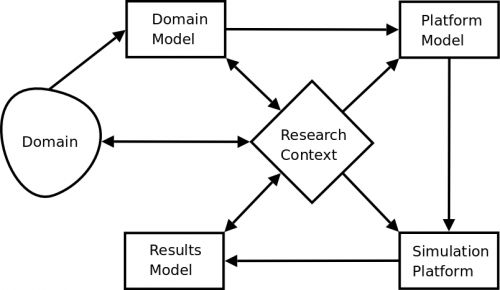
\includegraphics[width=\columnwidth]{cosmosProcess.png}
   %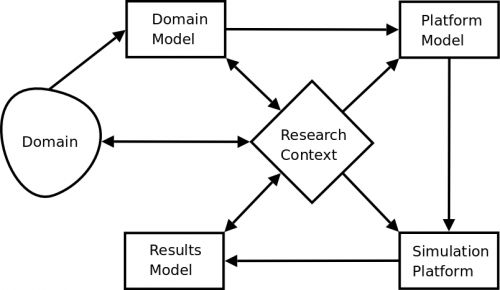
\includegraphics[width=\linewidth]{cosmosProcess.png}
  \caption{The Cosmos Process, after \cite{cosmosBook}}\label{fig:cosmos}
  %\Description{The 1907 Franklin Model D roadster.}
\end{figure}
Starting from the Domain, CoSMoS is predicated on close collaboration between a domain expert (a specific researcher or laboratory) and a developer (one or more simulation engineers).  Knowledge about the domain is always mediated by the domain expert, so that the simulation and its design represents a view that can be recognised and agreed by the domain expert.  Development proceeds by capturing what the simulation will do (a purpose or hypothesis, and key concepts and behaviours from the domain implicated in the real-world behaviour) in a domain model -- this is an agreed basis for simulation between domain expert and developer.  The simulation engineer assumes the lead at this point, devising a platform model from the domain model: this is typically a set of state diagrams that express the behaviour of first real and then computational agents, often complemented by other UML behaviour diagrams such as activity diagrams.  The development of the simulation platform is recommended to be as systematic as possible (plans to realise software using model transformation have not yet been fully realised \cite{workshop}).  Simulation experiments are run on the simulation platform and produce simulation results.  A simulation result can be compared to the real world, but, crucially, is not a real world observation.  Throughout development, a record must be kept of sources, assumptions, interpretations, design decisions, and other collateral information (the research context; this information is used to inform the analysis of simulation results and interpretation back to the real world.  Examples of research using CoSMoS, alongside domain experts in a range of immunology areas, can be found in PhD theses and associated papers (e.g. \cite{aldenPhD,moyoPhD,readPhD,williamsEAE} and other research from the former York Computational Immunology Laboratory).  These researches also demonstrate the use of argumentation \cite{AldenArg,cosmosBook} to document the basis of belief for the fitness for purpose of models, simulation, statistical and other analysis methods.

The CoSMoS outline gives us a basis for identifying where uncertainty arises in a domain, modelling and simulation, and a pointer to how different forms of uncertainty manifest and can be handled.
Figure \ref{fig:extended} extends the key products of the CoSMoS process (from Figure \ref{fig:cosmos},  showing all the activities contributing to the demonstration of fitness for purpose, the overarching quality management and argumentation that supports the use of a complex simulation in a research context.  

\begin{figure}[ht]
  \centering
  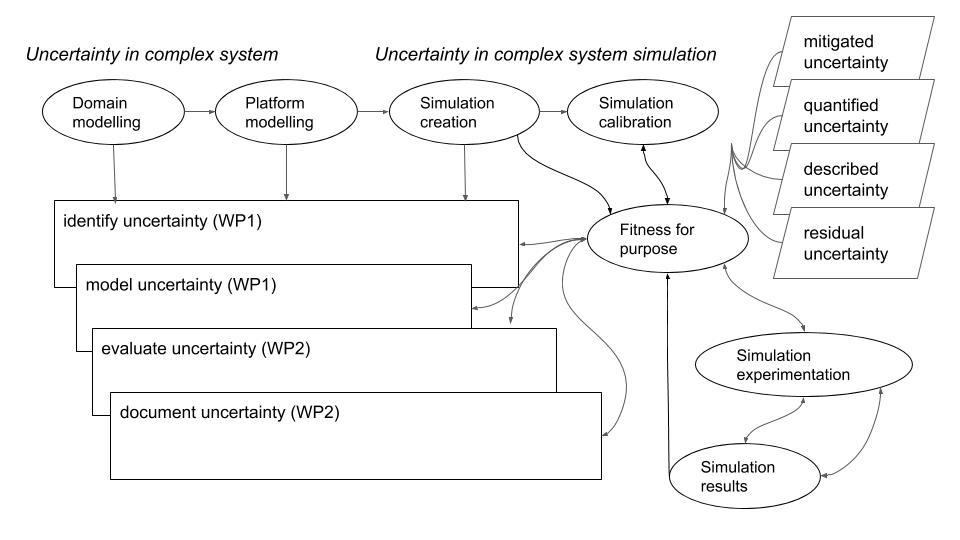
\includegraphics[width=\linewidth]{Process.jpg}
  \caption{Uncertainty and the Cosmos Process: ovals represent the CoSMoS products from Figure \ref{fig:cosmos}, with the additional steps required for demonstrating fitness for purpose and experimental use of the simulation; uncertainty-related activities are rectangles, and their outputs are parallelograms; arrows are indicative not comprehensive.}\label{fig:extended}
  %\Description{The 1907 Franklin Model D roadster.}
\end{figure}

Identification of uncertainties would be incremental, and can occur at any point.  We need to incorporate identified uncertainty into models, to evaluate their nature and effect, and to document our evaluation of the uncertainty.  During calibration and use of a simulator, we continue to identify, evaluate and document uncertainties. The outputs of our proposed uncertainty activities (parallelograms in Figure \ref{fig:extended}) comprise uncertainties that are amenable to quantification or description or are mitigatable, as well as residual uncertainties (known and unknown unknowns).  




% Whereas current software engineering research that is addressing design uncertainty focuses on techniques such as partial modelling \citep{Famelis2017} that enable initial uncertainties to be recognised and then successively engineered out, we will focus on capturing, recording, and analysing the effect of inherent uncertainty that is a necessary part of the simulated complex system.  We need ways to identify, and evaluate the effect of, uncertainties in the real and simulated systems.  


%_______________start of motivating examples ____________
\section{Examples of uncertainties}

To illustrate some of the origins and consequences of uncertainty, we present two motivating examples, which are not specific to any one research study but capture a range of our experiences in creating and using complex systems simulations.

\subsection{Motivating example 1: laboratory research simulation}

It is often the case that a biologist needs to understand an \textit{in vivo} process such as an  aspect of immune system development, but existing technologies limit their ability to observe the behaviours of the internals of a living organism: ethics limit what can be achieved with live subjects; even non-invasive techniques (e.g. external detection of the location and movement of ingested dyes) modify behaviours, either through chemical changes or through the consequences of stressing or anaesthetising the subject.  Simulation offers an ethically sound, repeatable, and extensively modifiable experimental platform, and, once sufficient knowledge (e.g. from \emph{in vivo} and \emph{in vitro} experimentation)  exists, can provide a route to confirm the feasibility of theories and a source and test-bed of new hypotheses.

Our example assumes that there is a clear hypothesis, but it can only be tested by perturbing or destroying a living organism.  A simulation developer -- typically a software engineer -- works with the biologist, using a principled approach such as CoSMoS to create a simulator \cite{aldenPhD,NACO14background}; they agree the design, and the compromises needed to digitise and execute the design.  The simulation uses suitable analogies of known cell mechanisms, and they agree that it is fit for its defined research purpose.  After calibration, experiments are run \emph{in silico}.  

Calibration and experimental results highlight differences between the simulation and the observed biology.  The differences could indicate uncertainties in the domain knowledge, but might equally be side-effects of design or implementation decisions -- or even statistical aberrations.  
The biologist and software engineer need considerable effort and expertise to understand and analyse the simulation results, and to relate simulation findings to the biological domain.  

Key research questions, relating to uncertainty in research simulations, are:
\begin{enumerate}
\item for each real-world concept, what is the initial assessment of uncertainty of domain knowledge?
\item for each simulation concept, how do design and implementation decisions diverge from the real world concept, and what additional uncertainty do these divergences introduce?
\item for each element of uncertainty, can the uncertainty be reduced (e.g. a simulation can test across a range to identify likely parameter values, which can be checked biologically); quantified (e.g. identify that a behaviour is observed with a particular probability; extrapolate from simulation results or reality); or simply described (e.g. we know that simulating a 3D reality in 2D introduces uncertainty but not much more).
\item can we evaluate and argue the reliability of simulation results?  Can we distinguish conditions under which results are likely to be reliable from those where we are less confident of the results (e.g. our PPSim \cite{aldenPhD,sim-pp} can reliably simulate formation of a Peyers' patch, but not the termination of formation or the distribution of patches).
\item how, and in what circumstances, can we measure the reliability of simulation results?  (e.g. when Simomics uses simulation in drug discovery, can it quantify reliability so that clients can focus their R\&D appropriately?)
\end{enumerate}

Addressing these key questions has the potential to provide clear and systematic understanding of sources and effects of uncertainty: (a) clear definition of scope, scale, purpose and simulation hypotheses; 
(b) guidance on where to focus activities to calibrate and test a simulator; 
(c) confidence in what the results reveal about the system and how results relate to real biological behaviours.
% will result in better understanding of what a simulation result means in relation both to the simulation process and the simulated domain.  Researchers will be able to distinguish between precisely known uncertainties and uncertainties that cannot be resolved, and will potentially identify critical uncertainties, areas where further research might make a significant contribution to understanding.  Specifically, addressing these questions : 

\subsection{Motivating example 2: robotics behavioural simulation}

Robotics uses agent-style simulation in development of behaviours of  individual robots and, particularly, of robot swarms. For instance, a roboticist creating an evolutionary algorithm works in simulation, eventually implementing either evolved behaviour or a successful evolutionary algorithm in an embodied system.  Similarly, robot swarm algorithms are typically created (or evolved) and tested \emph{in silico} before embodiment in swarm robots.  A roboticist designs the control software on a publicly-available simulation platform that encodes the mechanics and physics of the style of robot and the environment.  When evolving individual or swarm robot algorithms, the evolutionary algorithm are created and run in simulation, and then installed on actual robots.  

The behaviour of each real robot always differs both from the simulation and the behaviour of other instances of the same embodied robot.  The robotics term for this is the \emph{reality gap}.  Divergence arises from the uncertainties of modelling the robot and its environment and the uncertainties in the mechanics and set-up of real robots.  

It is futile to  try to engineer out uncertainty in robotics: real environments are complex and uncertain; robotic systems exploit the environmental and embodied uncertainties to evolve complex behaviour.  
Key research questions relating to uncertainty in robotic evolution, are:
\begin{enumerate}
\item can we identify systematic variation between simulation and embodiment (e.g. for one type or robot or one type of environment), and can we quantify or describe the variation?
\item can we identify and quantify the effects of the different characteristics of uncertainty in the real robots and of noise introduced to a simulated robot or swarm?
\item can we identify characteristics of uncertainties of the real environment that are used by embodied robots or swarms in ways that are different to the noise introduced to a simulated environment, and can we quantify these effects?

% ADDED BY AS 30/Apr
\item can we identify characteristics of uncertainty in both real and simulated environments that provoke first-order effects (e.g. generalization or noise-robustness) in evolutionary systems? 
\item can we reduce the reality gap such that simulation becomes a more effective design tool?
\end{enumerate}

A clear and systematic understanding of the sources and effects of uncertainty in robotic systems would (a) allow calculation of uncertainty bounds that can be considered in both evolution and embodiment; and (b) provide guidance on how simulations can be tuned to a better representation of a specific context and environment.

%_______________end of motivating examples ____________


\subsection{Examples: commentary}

In the domains of both motivating examples, complexity and uncertainty are inherent.  Biological behaviour is complex on many levels, and complexity is inherent to the context of the behaviours under investigation.  The mechanics and environment of an embodied robot or robot swarm are inherently complex, and it is infeasible to express all the complexities of realities in a simulation.  In both domains, a systematic way to capture and express uncertainty would be of benefit in simulation design, analysis, use, and comparison with (or embodiment in) the real world.  

\section{Related work}\label{sec:related}

Uncertainty has been widely researched, but mainly to eliminate or control it.  By contrast, in simulating complex systems, we need to retain and incorporate uncertainty, and to understand the influence of uncertainty on simulation experimentation. 

There are many existing ontologies and taxonomies of uncertainty, and some metamodels, which offer a starting point for identification or classification of uncertainty.  There are also many approaches for quantification or mitigation of uncertainty.  %We will develop metamodels of uncertainty in our chosen domains.  Our research draws on existing uncertainty research in many domains, and on identification, classification and management of uncertainty.  We will develop ways to document, identify, model, and evaluate the effect of uncertainty in complex simulations.

The process of identifying uncertainty is something of a circularity: to detect uncertainty, we need to know what sort of thing we are seeking.  A common indicator of uncertainty is the implicit or explicit assumptions made in modelling.  

The most prominent protocol for agent modelling, originating in the ecological community, is the ODD (Overview, Design concepts, Details) Protocol \cite{ODD2006,ODD-2020}.  ODD is recommended by agent-based communities such as CoMSES OpenABM\footnote{\url{https://www.comses.net/}}, along with data protocols, such as the FAIR principles \cite{FAIR2016}.  ODD originated as a protocol to improve the scientific reproducability of simulation results, and provides a template to document the design and rationale of the simulation.  However, there is no explicit recording of assumptions, only the source or rationale of design decisions.  The protocol has nowhere to express or explore what is not definitively known in the domain, design or use of the simulation.  Similarly, the FAIR principles focus on complete and consistent documentation of (meta)data, but do not consider documentation of data uncertainties.   

The CoSMoS process \cite{cosmosBook}, by contrast, puts emphasis on identifying and recording assumptions, and on arguing the fitness for purpose -- and thus also the limitations -- of the simulation.  It has been argued that the ODD protocols and CoSMoS are complementary \cite{cosmos-odd}, but there has been no attempt create an alignment.


\subsection{Identifying and evaluating uncertainty} 

There are many existing attempts to define uncertainty.  Jousselme et al. \cite{unc-sap} review many existing hierarchies and ontologies, in their search for a comprehensive set of definitions on which to build an understanding of uncertainty.  Basing their contribution on situational analysis, they distinguish various types, ranging from ignorance (a state of mind) and uncertainty (a consequence of limitations in observation).  

Padulo and Guenov \cite{unc-ced}, working on engineering design, also present an extensive review, and crucially  note that design decisions are not rationally-justified decisions taken once all facts and options are available, and that the design process itself results in a growth of knowledge -- and, presumably, a reduction in uncertainty.  Padulo and Guenov provide a useful high-level summary, in which the design problem is seen as separable into uncertainty about and uncertainty within the problem (Figure \ref{fig:design}).  Uncertainty about the problem includes issues such as assumptions, values and external influences, whilst uncertainty within the problem comes from experts, data, models, design approaches and imposed standards.

\begin{figure}[ht]
    \centering
    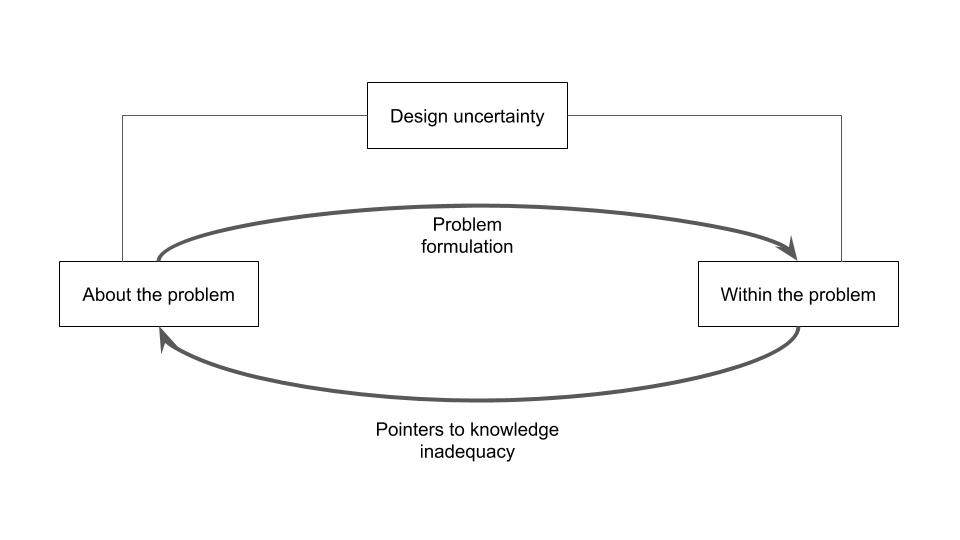
\includegraphics[width=\columnwidth]{design.jpg}
    \caption{Classes of design problems relating to uncertainty, summarising the scheme of Padulo and Guenov \cite{unc-ced}}
    \label{fig:design}
\end{figure}

Both the above works touch on the issue of quantification of uncertainty. Knight \cite{knight2012risk} separates quantifiable effects, which he labels \emph{risk} and describes as randomness expressed by probability and statistics, from uncertainty, which is any other sort of unknown effect.  Lo and Mueller \cite{physEnvy} extend the classification of uncertainty to \emph{fully reducible}, \emph{partially reducible} and \emph{irreducible}, noting that what is irreducible in one domain (and with the current state of knowledge) may be (partially) reducible in others.  

Many researchers define uncertainty as \emph{systemic} or \emph{epistemic} uncertainties, denoting things that could be known but are not, such as missing parameters, variables, structures, unknown distributions or imprecise algorithms \cite{unc-schunn}.  There is extensive research on approaches that can turn systemic or epistemic uncertainties into \emph{aleatoric} uncertainties -- things that are not precisely known but vary in ways that can be expressed in statistics (e.g. \citet{unc-bayes}) or mathematics (e.g. \cite{unc-ober,unc-PATELLI}), in order to quantify and manage reducible uncertainty. For example, Kennedy and O'Hagan \cite{kennedyBayes} present Bayesian approaches to calibration for seven types of uncertainty.  

Identification of uncertainty is inherent in engineering disciplines that seek to mitigate or control uncertainty (e.g. MIT Uncertainty Quantification Group;  aeronautic uncertainty \cite{unc-Park,unc-ZHEHAN,unc-SCHAFFER}; sources of uncertainty in self-adaptive systems \cite{Esfahani2013}).

A more colloquial approach is to label uncertainty as known unknowns and unknown unknowns.  However, within each of these categories, there are reducible and irreducible uncertainties, quantifiable, qualifiable (or describable) and merely identified uncertainties.


\subsection{Modelling uncertainty} 
 
There has been growing interest in modelling uncertainty, spearheaded by an OMG call for proposals and the OMG Uncertainty group\footnote{\url{http://www.omgwiki.org/uncertainty/oku.php?id=start}}.   The work includes a draft metamodel of uncertainty in cyberphysical systems \cite{unc-RFP}.  The focus is on capturing the (un)certainty of the modeller by expressing beliefs about information.  The state of the art is captured clearly by Vallecillo, in his keynote presentation to QUATIC2019\footnote{Modeling and Evaluating Quality in the Presence of Uncertainty, \url{https://www.slideshare.net/avallecillo/modeling-and-evaluating-quality-in-the-presence-of-uncertainty}}.  Vallecillo recognises the wide range of classifications of uncertainty, and  summarises the origins of uncertainty as comprising: under-specification; lack of knowledge; lack of precision; imperfect, incorrect or missing information; approximation; indeterminacy; and different interpretations of the same information by different people. 

\subsection{Arguments acknowledging uncertainty}
A potential complementary approach to modelling uncertainty through belief is used in critical systems engineering and in the CoSMoS simulation approach.  Rather than representing uncertainty directly in engineering models, an argument that acknowledges the weaknesses of the models is created.  

Argument use in critical systems engineering is encapsulated by safety case argumentation: for example, ISO61508(general), ISO26262(automotive), and DO-178B(airplane) require documentation of “Safety Cases”.  A typical example, the safety of aircraft systems, is presented as an argument over hazards and mitigations \cite{kelly2004systematic}.  The structure of arguments is most commonly presented using a notation such as the Goal Structuring Notation: a claim is asserted, with associated assumptions and elaborations; a strategy for evaluating the claim is chosen; sub-claims and strategies are stated; and eventually evidence supporting sub-claims is presented, such that the combination of all evidence amounts to a sufficient demonstration that the claim is met \cite{GSNStandard}.  The arguments allow manufacturers to support the general assetion that the risk associated with their system is \emph{as low as reasonably practicable}.


The CoSMoS team and York Computational Immunology Group has adapted argument notations to present the rationale for a belief in the fitness for purpose of complex systems simulations \cite{andrews2008simulating,AldenArg,Alden20141059}.  Arguments of fitness for purpose can be created for, for instance, models, implementation (design decisions), analysis techniques (e.g. statistical tests), and experiments.  Like a critical systems argument \cite{LevesonReuse}, the validity of the argument depends on the current context and use of the simulation: adaptation or reuse requires a revisiting of fitness for purpose.

\subsection{Tools}

There is a growing range of tools to support the various facets of complex simulation engineering.

It has long been acknowledged that uncertainties of mapping domain models through to a simulation can be partially addressed by domain specific modelling languages and workflows \cite{polackCEC,cosmosBook}.  Early work used metamodelling to define domain specific modelling approaches (e.g. \cite{polackMOTPW}), whilst several initiatives now seek to develop  domain specific modelling languages (DSMLs) for simulation \cite{workshop}.

Tools exist to support systematic calibration, sensitivity analysis, and statistical analysis of experimental results.  For example, Spartan\footnote{\url{https://www.kieranalden.info/index.php/spartan/}} \cite{spartan,spartan-sim} is an R-based package of statistical techniques specifically designed to explore the relationship between a complex research simulation and the real-world.  As such, many of its techniques focus on analsyis and reduction of uncertainty in complex systems simulations.  ASPASIA\footnote{\url{https://www.kieranalden.info/index.php/aspasia/}} \cite{aspasia} supports analysis of simulated biological behaviour that depends on an intervention, and the concomitant issues of calibration, which introduce uncertainty in the interpretation of experimental results -- e.g. in assessing the extent to which an alteration in behaviour can be attributed to the intervention alone.  Clarity on the classification and identification of uncertainty can lead to better application of the techniques for calibration, sensitivity analysis and statistical analysis of results supported by these tools.


A range of commercial tools to support documentation, argumentation and analysis of simulators (notably the virutal laboratory and associated tools offered by Simomics Ltd\footnote{\url{tools originating in the work of the CoSMoS team and York Computational Immunology Lab; https://www.simomics.com/offerings}}).  Such tools already provide means to document uncertainties, but need to be able to apply the classification and evaluation of effects of uncertainties. 

Whilst most of the tools identified relate to research simulations (and specifically, research in immunology), some have been adapted for robot simulation and engineering.  For example, the York Robotics Lab has developed RoboSpartan\footnote{\url{https://www.york.ac.uk/robot-lab/robospartan/}}, to support optimisation of the behaviours of robotic systems and targeted experimentation in hardware, specifically:
\begin{itemize}
    \item automated parameter value sampling and result analysis for uncertainty and sensitivity analyses;
    \item generated simulation configuration files;
    \item generated execution scripts;
    \item surrogate model generation, for use where a model analysis proves intractable;
    \item support for evolutionary and Bayesian computation techniques to identify parameter regions giving rise to desired behaviours.
\end{itemize}




\section{Discussion: uncertainty in complex system simulation engineering}


To advance the state of the art in complex systems simulation, we need to bring together learning from a wide range of uncertainty research, identifying how each can be used in complex systems simulation engineering, embodied here in the CoSMoS process \cite{cosmosBook}.  The goals are to  enable identification, modelling, evaluation and documentation of uncertainties and their effects.  

A classification of types of uncertainty that applies across complex systems simulation engineering needs to build on the work of authors such as Padulo and Guenov \cite{unc-ced}, Jousselme et al. \cite{unc-sap} and the OMG Uncertainty Group.  However, there is a need to go beyond a belief- or structural-analysis-based approach.  In complex systems simulation engineering, there are definitively-known uncertainties, such as parameters whose absolute value is unknown but whose range or distribution of values is not disputed.  These uncertainties are distinguishable from uncertainties that are known but not quantifiable, such as the effect on simulation of digitising space and time, and those only identifiable by  observation (e.g. a systematic but unexplained divergence between observed and simulated behaviour).

Once a classification of the generic uncertainties of complex simulation engineering is established, we need to understand how the classification applies and adapts in particular complex domains and on specific simulation subjects.  There will, for instance, be variations in forms and instances of uncertainty  manifested between and within research domains (e.g. uncertainties typical to simulated immunological behaviours will differ from uncertainties in simulations of collective human behaviour), whilst engineering simulations (here, for swarm robots and evolutionary robotic design) will manifest different variants of uncertainty to research simulations.

Following on from identification and classification of uncertainty, researchers can start to generalise analysis and treatment of uncertainties.  As in other domains some types of uncertainty could be reduced or eliminated, though the engineering value of reducing uncertainty is an important consideration: for instance, if more certainty in parameterisation or agent interaction reduces the number of runs of a simulator need to achieve statistically valid results, the cost of the increased certainty needs to be weighed against the cost of each simulation run.  If it takes significant effort (e.g. undirected laboratory exploration) to increase certainty of parameters or interactions, but each simulation run takes milliseconds, and 10 000 runs is sufficient to achieve statistically reliable results, the cost of certainty is almost certainly too high.  Conversely, if a tool-based calibration that takes a few hours to complete reduces the number or speed of execution runs so that  experimentation time (\emph{in silico}) reduces from months to hours, then the certainty-increasing intervention is likely to be cost-effective.  Cost-effectiveness may also depend on the use of the simulation results.  For instance, in a multi-million dollar drug development programme, a few days, or even months, spent improving the precision and reliability of a simulation of complex interactions with the selected drug(s) is likely to be feasible; the same reductions of precision in a laboratory research simulation where outcomes can be quickly validated \emph{in vivo} or \emph{silico} would likely not be cost-effective.  In many cases, we anticipate that greater effectiveness will come through  identifying, evaluating and documenting the uncertainties, than through actions taken to reduce simulation uncertainty.  

There is ample literature on handling uncertainties that are amenable to quantification.  These range from creating statistically valid results sets to determine the statistical significance of results, to using known distributions to determine the values of specific parameters in each agent in a simulation \cite{read-stats,spartan-sim,spartan}. 
Two examples, from our existing research simulations, are as follows.
\begin{itemize}
    \item In research to tie down the specifics of uncertain low-level behaviours known only from limited time-interval observation in the laboratory, simulation experimentation was able to pinpoint the timing and extent of interactions implicated in Peyer's Patch formation, which were subsequently tested and accepted in the laboratory \cite{aldenPhD,sim-pp}.
    \item In research to isolate values for  parameters approximated by  the domain expert, an AI search over the set of uncertain parameters yielded sets of candidate values; working with the domain expert, this led to identification of the best real-world match, and specifically to identification of one parameter whose uncertain value was then shown to have caused divergence between the simulated and real observations; the result was again validated in the laboratory \cite{garnett2010computer}.
\end{itemize}

However, we must recognise that a statistical characterisation does not offer understanding: the uncertainty of values or computational behaviour may be reduced, but uncertainty remain in how the real world achieves an observed behaviour. 
Furthermore, it is a feature of complex system simulation (whether for research or engineering) that the models and implementation actually characterised the combined effect of many unknowns. Where we use quantitative modelling or analysis of uncertainty, there is a critical need to record the rationale and likely side-effects of quantification.  Argumentation of fitness for purpose already captures some information about uncertainties, but needs to be adapted to systematically record uncertainty.  Since an argument of fitness for purpose is only a structural summary of the rationale for our confidence in simulation, we also need a systematic process and template for  documenting what we do know about each type of uncertainty, whether related to the domain, simulation, experimentation or results.

An ultimate goal would be to determine system-level uncertainty: to be able to combine known and unknown uncertainty evaluations in a way that allows a summary of the overall effect of uncertainty, and an evaluation of the consequent reliability of results or observations on simulation. 

\section{Conclusions}

Uncertainty pervades any complex system, whether in reality or simulation.  There is a wealth of writing on the classification of uncertainty, but rather less on domain-specific uncertainty, its identification, description and evaluation.

Systematic complex systems simulation engineering, as advocated by CoSMoS, provides a basis for exploring how uncertainties in research and engineering domains and simulations can be identified, modelled, evaluated and documented.  The state of the art in other areas of uncertainty research offer directions to take in relation to mitigation, quantification and description of uncertainty.  However, we recognise that, when working with uncertainty, there are likely to be residual uncertainties (such as systematic but unexplained differences between simulated and observed behaviour) that can only be recorded.

An approach to manage uncertainty in complex systems simulation and experimentation needs to address not just design practices but also the design or experimentation, rationale or fitness for purpose, and analysis of results.  In these areas, existing tools can be enhanced to model and address aspects of uncertainty.

We envisage that the management of uncertainty in research and engineering simulation of complex systems would have direct application alongside existing simulation and support tools in reducing    development time and costs.  For instance, the pharmaceuticals industry now employs simulation in drug discovery, but lacks a way to record and evaluate the unknowns and uncertainties of the domain and simulated system: clear, partly-quantifiable, evaluation of the limitations and caveats of the simulation will help to reduce costs and improve reliability of simulation use in drug discovery.

In robotics, improved understanding and observance of uncertainty should lead to  simulation platforms that better represent the context and environment of individual or swarm robots, prior to embodiment.  Capturing and analysing cumulative uncertainties in the simulator and domain has the potential to make robotic systems development more effective; we can also support simulation of service or maintenance robotic systems in situ, exploring the evolved behaviour, safety, and reliability of robots in realistic domains with improved (and sometimes quantifiable) likelihood of successful embodiment.

  \bibliographystyle{ACM-Reference-Format}
  \bibliography{bibfile}
\end{document}
